\section{Theory}

\subsection{How does Augmented Reality work?}

\subsubsection{History of AR}

\subsubsection{S.L.A.M.}

\subsubsection{Depth tracking}

\subsubsection{Cameras}

\subsubsection{Other inputs}
Compass, Gyroscope, Accelerometer  etc.

\subsection{What Machine Learning methods are there?}
There exists many different machine learning techniques out there today. Due to its high effectiveness and relevance, for this report we are going to focus on the highly popular method of artificial neural networks.
This is a proven method for working well with images (Convolutional neural networks) and is therefore a highly 
relevant technique for this project.

\subsubsection{Perceptron}
A perceptron is the simplest form of the neural network. It has a set of inputs and an output.
The perceptron first sums up all the input values, x, multiplied with the weight value, w.
After that it passes that sum through an activation function. This activation function can be everything from a simple f(x)=x to the more complex sigmoid function, depending on the need. More on this in the upcoming section.

\begin{figure}[hbtp]
\begin{center}
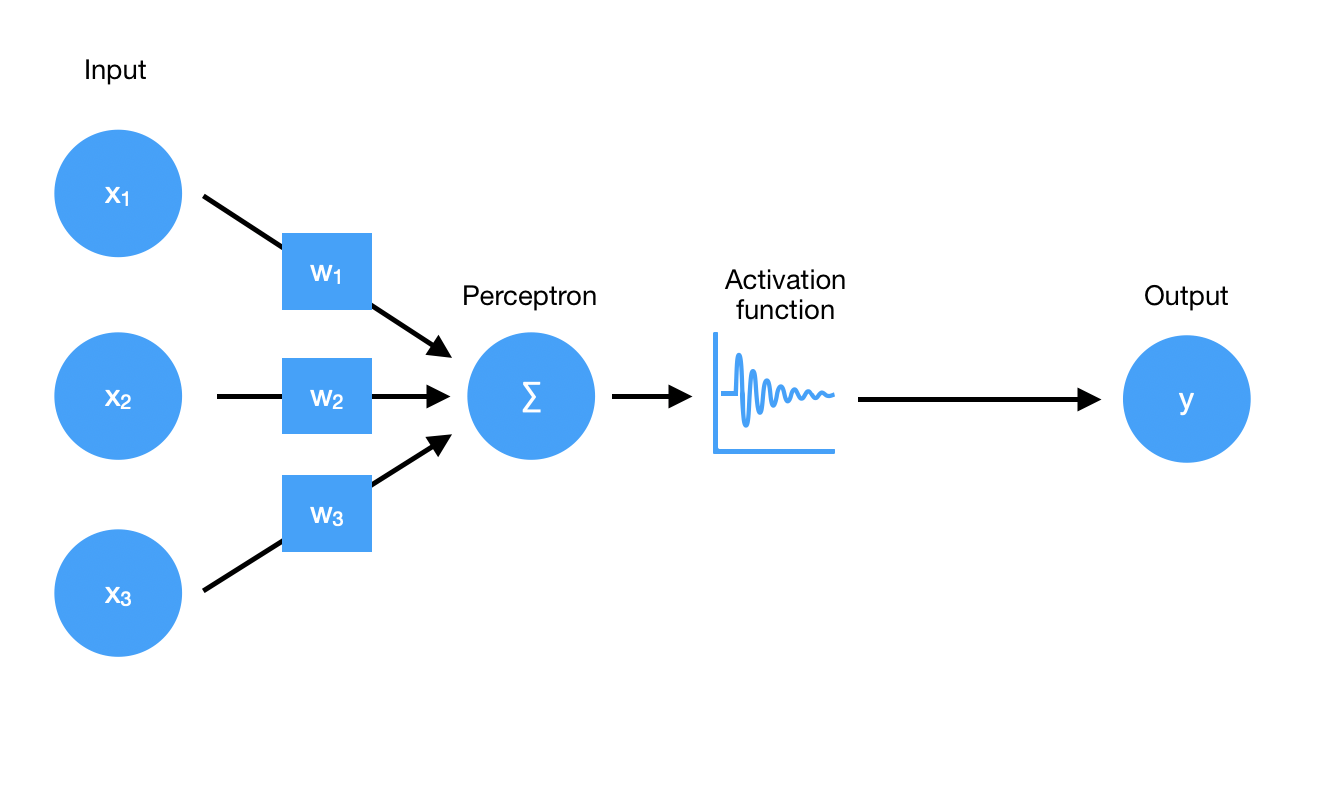
\includegraphics[width = 0.75\textwidth]{./Images/perceptron.jpg} 
\caption{An illustration of the perceptron, the simplest version of a neural network.}
\end{center}
\end{figure}

A bias also exists in every node which is not based on any input. The bias function in the perceptron is similar to what the m in y = kx + m does. It gives the function the ability to move up and down in the graph for more possibilities of splitting the data set. The bias is usually disregarded when illustrating the perceptron.

The perceptron only has the ability to draw a single line and thus is only able to split simple data sets.

*Formula for the output of the perceptron*

\subsubsection{Activation functions}

ReLu
Tanh
Sigmoid
Softmax

\subsubsection{Loss/Optimizers}

Mean squared

SGD
Adam
Nadam

\subsubsection{Layers}

\begin{figure}[hbtp]
\begin{center}
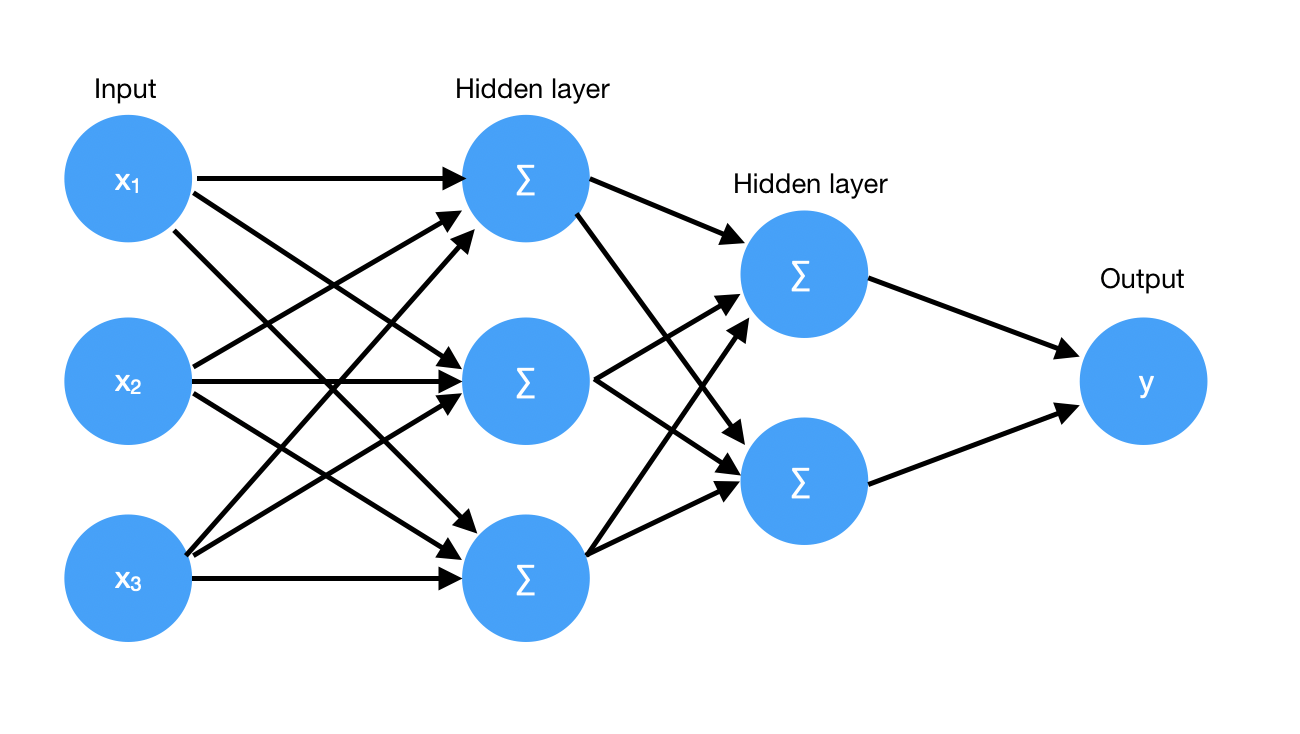
\includegraphics[width = 1.0\textwidth]{./Images/fully_connected.jpg} 
\caption{Two fully connected layers. One with 3 neurons and one with 2 neurons.}
\end{center}
\end{figure}

With more layers and more neurons the networks parameters and complexity begins to grow. So does also the training time, size of the model and the cost for doing predictions. Thus, these networks are capable of describing much more complex data sets. But as a result of that, the risk of overfitting (The act of describing the training data set too well so that new data sets will not get recognized. More on this soon.) becomes much greater. That is why a complex network is not always wanted.

\subsubsection{Overfitting}
When training a neural net, one needs to be careful not to train the model too much or overfitting is likely to happen. Overfitting is when a model gets REALLY good at predicting the data that it is training on but fails to predict accurately on new data. This is because it starts to pick up too much on detail or in some instances even noise. For this reason it fails to pick up the general trends, which is more valuable. 

\begin{figure}[hbtp]
\begin{center}
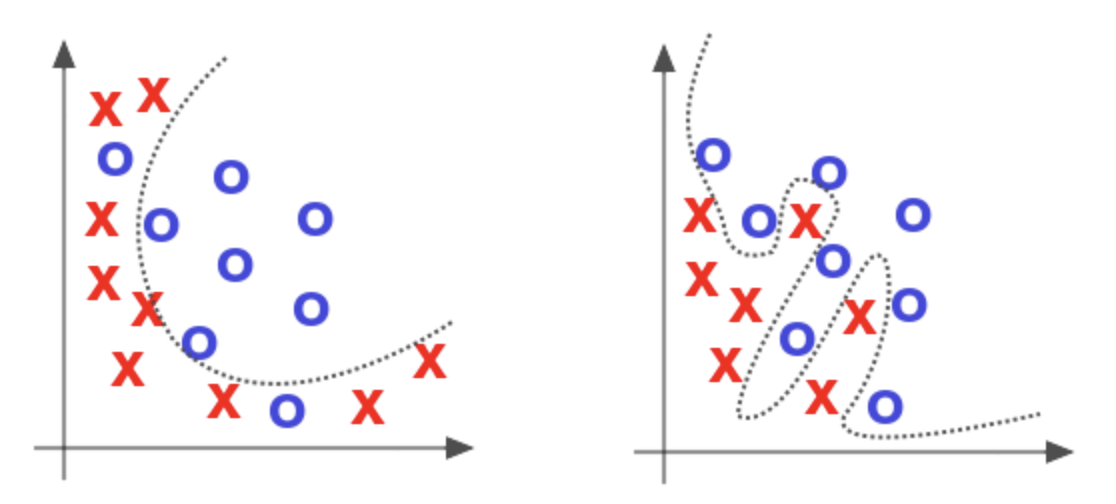
\includegraphics[width = 1.0\textwidth]{./Images/overfitting.jpg} 
\caption{Overfitting of a dataset. On the left is a accurate trained model, on the right is an overtrained model. Image taken from OReilly.com}
\end{center}
\end{figure}

\cite{overtraining}

There are tricks for combating overfitting. They usually involve trying to limit the size of a small amount of weights.
The hypothesis behind this is that if a weight is much larger than the rest it also has much more influence over the final prediction. That way, a small detail in the data can have much more influence than the general trend.

One way to do this is to cut random connections between layers during epochs, usually by specifying a certain amount that is going to be cut.
This way, the model is not relying on a small number of nodes to make the correct predictions. This method is called dropout.

Another way is to introduce random noise on a layer during training. This works because if a node with a large weight receives noise, it will be heavily amplified and probably give a false prediction.
When doing this, Gaussian noise is usually implemented, which is basically random noise with a gaussian distribution.

To force the model to keep weights small, one way is to add a penalty to the loss for every weight based on its size. 
This is called weight regularisation and is widely used and exists in two forms, L1 and L2.
L1 simply adds the weights size multiplied with an l1 term that is chosen by the designer.
The other, L2, is to do the same but in this case square that value. This has the effect of making values over 1 even bigger and values less than 1 smaller.
In that way, it doesn't affect the loss as much as L1 when not being overtrained. L2 is also called weight decay and is the more common method of the two.

One important thing to point out is that all these methods mentioned so far are only active during training and is not doing anything when making real predictions.


If lots of training data exists, the ensemble technique could be a good way to go. This technique divides the training data into more smaller sets and trains a model for every data set.
The final prediction is then an average of the predictions of all the models. This technique works because if the model is highly overtrained in a certain direction, chances are that the other networks will drown out this result by the many other models.

It is kind of like when someone has an off pitch in a big choir. If there are many other singers, this off-pitch will not be noticed very much.

\begin{figure}[hbtp]
\begin{center}
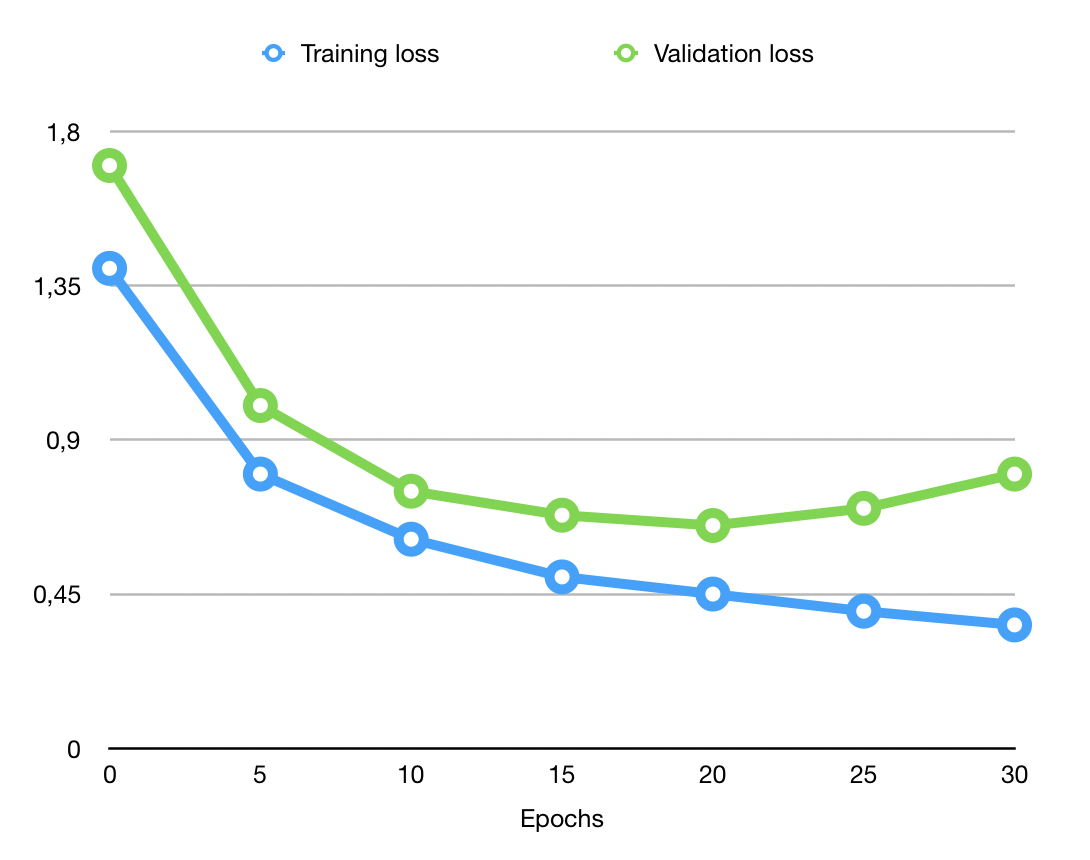
\includegraphics[width = 0.75\textwidth]{./Images/early_stop.jpg} 
\caption{A graph showing when to do an early stop. The graph shows the total loss over trained epochs. Notice that the validation starts to increase again somewhere after epoch 20.}
\end{center}
\end{figure}

The final technique is called early stopping and is based on validating the model after every epoch and stopping the training when the validation loss, or some other criteria, is not improving anymore.

\subsubsection{Deep Neural Networks}
% Write about how Deep Neural Networks work and how it's applyed to image classification

\subsubsection{Transfer Learning}
% Write about the theory behind Transfer Learning


\subsection{Object Detection without machine learning}
% Write about feature based detection and segmentation

When trying to detect objects in a still image we have looked into two main methods. One typical way is to try and look for patterns or features in the image.
Either a specific image can be matched within the larger image or a series of features can be found.
An example of the latter is Haar features which is used in the Viola-Jones for face detection. Using the image integral (which is the summation of pixel values in a specific region) different features can be obtained.

\begin{figure}[hbtp]
\begin{center}
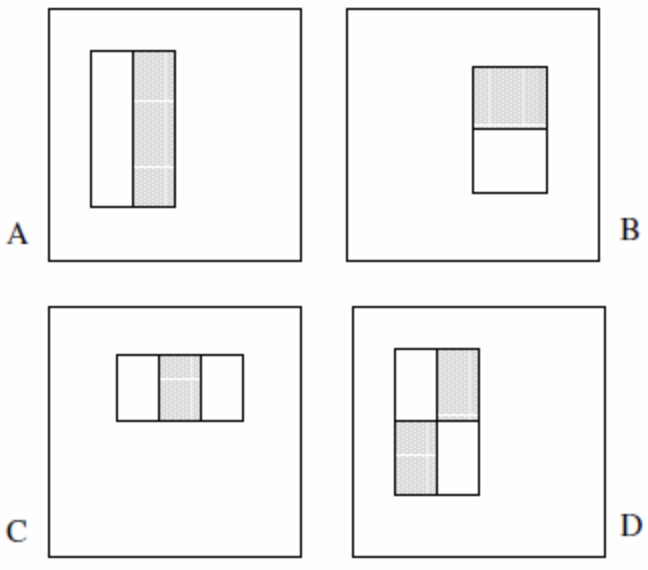
\includegraphics[width = 0.75\textwidth]{./Images/viola-jones.jpg} 
\caption{A set of Haar features used to detect faces in the Viola-Jones method. The pixels in the white regions are summed and subtracted with the pixels in the black region. The algorithm will later decide if a specific feature has been found or not, depending on obtained value.}
\end{center}
\end{figure}

This method is based on the fact that every face shares some basic similarities. Even objects of the same type can share some similarities.\cite{violaJones}
\\\\
Another way to find objects in an image is to try to classify each pixel as either background or foreground, usually referred to as Foreground/Background-segmentation. This usually requires some background knowledge of how the background usually looks like, for example, if the background is grass or a concrete floor.

One of the most basic functions for separating background and foreground is the flood fill method.
Anyone that has used Paint for Windows knows exactly what this one is. It fills a segment of similar pixels with the same color. This method works best on one backgrounds with only one color.
Online there are many different variations but they all accomplish the same goal.\cite{floodFill}
\\\\
Mathematical morphology

Edge detection

Histogram equalisation
\\\\
One possible way of detecting objects in an image is to use depth data, or RGB-D.
A tool that typically comes to mind when reading about depth data is the Kinect camera
for Xbox.

On the iPhone X, depth data can be captured by either True Depth on the front camera or with the dual cameras on the back. The True Depth camera works by having a dot projector emit light dots (mainly on a face which is why this feature is found on the front camera) and picking those dots up with an infrared camera.

The dual camera on the back works by taking two photos and comparing those to find the pixel shifts of the same objects. The distance is calculated by (pixelShift / (pixelFocalLength * baselineInMeters)) and gives the unit in (1/meters). It is the same principal to how we humans see distance by having two eyes pointing the same direction. \cite{depthMap}

However, obtaining the depth data from the dual cameras in real time is not possible since it requires too much computational power. This unfortunately makes it impossible to use in an ARScene and thus not possible for this project.\\

Despite all the available methods above, object detection without machine learning is still very tricky. These methods works best when the images are in an controlled environment, typically industrial, like finding screws on a white background.
When the environment is a more casual place tough, like recognizing furnitures indoors, the task becomes much more difficult. For this reason, object detection with pure algorithms is not very common in household applications. Instead object detection with machine learning methods such as RCNN networks are much more common nowadays.

\subsection{Object Detection with machine learning}
% Write about how one can do object detection by the use of ML

Big advantages with this is that classification and detection can be done in the same step. For this project that is really desirable.

\subsubsection{RCNN and its different forms}

\subsubsection{YOLO}

\subsection{Object recognition with machine learning}


\newpage
